\documentclass[12pt]{article}
\usepackage{amssymb,amsfonts,amsthm,mathtools,float,color}
\usepackage{caption,subcaption,tikz,gensymb,pgfplots}
\usepackage{graphicx}
\graphicspath{ {images/} }
\pgfplotsset{compat = newest}
\DeclarePairedDelimiter\ceil{\lceil}{\rceil}
\DeclarePairedDelimiter\floor{\lfloor}{\rfloor}
\usepackage[hmargin=1in,vmargin=1in]{geometry}
\newcommand{\si}{\sigma}
\DeclareMathOperator{\lb}{lb}
\DeclareMathOperator{\ls}{ls}
\DeclareMathOperator{\rb}{rb}
\DeclareMathOperator{\rs}{rs}
\DeclareMathOperator{\LB}{LB}
\DeclareMathOperator{\Max}{Max}
\DeclareMathOperator{\LS}{LS}
\DeclareMathOperator{\RB}{RB}
\DeclareMathOperator{\RS}{RS}
\DeclareMathOperator{\hook}{hook}
      \theoremstyle{plain}
      \newtheorem{theorem}{Theorem}[section]
      \newtheorem{lemma}[theorem]{Lemma}
      \newtheorem{corollary}[theorem]{Corollary}
      \newtheorem{proposition}[theorem]{Proposition}
      \theoremstyle{definition}
      \newtheorem{definition}[theorem]{Definition}
      \theoremstyle{remark}
      \newtheorem{remark}[theorem]{Remark}
      \theoremstyle{plain}
      \newtheorem{conjecture}{Conjecture}[section]
\def\vs{\vspace{1\baselineskip}}
\def\svs{\vspace{.5\baselineskip}}
\def\bs{\vspace{5\baselineskip}}
\def\zik{\mathcal{Z}_{i,k}}
\def\setzik{\{\mathcal{Z}\}_k}
\def\Z{\mathcal{Z}}
%\newcommand{\tre}[1]{\textcolor{red}{}}
\newcommand{\tre}{\textcolor{red}}
\newcommand{\tbl}[1]{\textcolor{blue}{}}
\newcommand{\tgr}[1]{\textcolor{green}{}}
\DeclareMathOperator{\WLB}{WLB}
\DeclareMathOperator{\WLS}{WLS}
\DeclareMathOperator{\WRB}{WRB}
\DeclareMathOperator{\WRS}{WRS}
\DeclareMathOperator{\WF}{WF}
\DeclareMathOperator{\W}{\mathcal{W}}
\def\zik{\mathcal{Z}_{i,k}}
\def\setzik{\{\mathcal{Z}\}_k}
\def\Z{\mathcal{Z}}
\def\M{{\bf M}}
\def\l{\ell}
\def\multiset#1#2{\ensuremath{\left(\kern-.3em\left(\genfrac{}{}{0pt}{}{#1}{#2}\right)\kern-.3em\right)}}
\newcommand{\Rtil}{\widetilde{R}}
\newcommand{\LBtil}{\widetilde{\LB}}
\newcommand{\LStil}{\widetilde{\LS}}
\newcommand{\RBtil}{\widetilde{\RB}}
\newcommand{\RStil}{\widetilde{\RS}}
\newcommand{\gauss}[2]{\genfrac{[}{]}{0pt}{}{#1}{#2}} 
\newcommand{\TODO}{\tre{TODO!!!!!!}}
\newcommand{\interesting}{\tre{SUPER INTERESTING\\}}
\newcommand{\figureout}{\tre{Need to figure this out\\}}
\newcommand{\N}{\mathbb{N}}

\begin{document}
\title{Playing Pong with Deep Reinforcement Learning}
\author{Bobby Dorward, Ryan Wilson, and Eric Bell}
\maketitle

\section{Introduction and Background}
%type here
%percent signs are comments
%type \section{section_name} for a new section
%compile to see what it looks like
\par 
The history between artificial intelligence and gaming is long standing because short term choices give rise to long term sophistication.  For example, the moves possible in the game of Go are few, yet it took one of the most sophisticated machine learning algorithms to date to be able to perform sufficiently at this problem.  We aimed to revisit this relationship between machine learning and gaming in order to gain  facility with how machine learning, specifically deep neural networks, are used.
\par
We have trained our neural network through reinforcement learning, specifically through an implementation of Q-learning. [BOBBY PLS WRITE THIS SECTION SO ITS THE MATHINESS YOU WANT]
\par
Our algorithm interacts with the game through the OpenAI Gym[1], an environment that allows the programmer to interact with Atari games (as well as a few other simulations) such that a machine learning algorithm can be trained to play the game ("solve" the problem).  What this entails is that the Gym allows us to extract pixel data from the game, signal actions for the AI to take on a frame-by-frame basis, and collect feedback used to train the algorithm.  Our original goal when starting this project was to apply this network to the "DoomBasic-v0"[2] but due to limitations, we decided to start with the simpler "Pong-v0"[3] environment.  This environment runs a typical game of pong: a ball bounces between two paddles and one player scores when the ball hits the opposing side of the screen.  The two players continue until someone scores 21 points, after which the game ends.
\section{Data}
\par
As previously mentioned, the data we used as input into our deep network was the pixel data of the environment.  Each pixel is represented as an array of three elements, representing the three channels of an RGB pixel.  Neural networks by nature are memory-intensive data structures due to the large amount of nodes and connections they contain.  This is especially true when one uses a more complex derivative of a neural network, such as the deep neural networks we have implemented.  Therefore, despite our best efforts to make our implementation generic and applicable to many different environments, we had to make pong-specific alterations to our data to streamline the size of the network and make it runnable on the resources we had available to us.
\par
The first change we made was to grayscale the pixel values, thereby cutting the data we need to put into our network by three.  Essentially what this means is that we have averaged the three values of the RGB channel into one value for each pixel.  Next, we cropped the images being given to us by the OpenAI Gym in order to exclude all the pixels on the screen that weren't directly relevant to the frame-by-frame progression of the game: the scoreboard, the white edges, and the padding behind each paddle was cropped to minimize the input count of the network.  (Downsampling/Pooling?) Through this preprocessing, we were able to reduce the amount of inputs being taken for each frame to 20,800.
\par
Finally, since the game of pong does not consist of still images, but rather gains meaning through the motion of the game objects (two paddles and the ball), we needed to capture this motion using the pixel data.  We achieve this by extrapolating a difference frame (shown below) between each subsequent pair of images, in which we subtract the first image from the second image.  Through this, we can train the algorithm with data that represents where the game objects have been and where they're going, zeroing out any unmoving (and thus irrelevant) pixels in the process.  It is because of these difference frames that we have limited the action that our AI can take; instead of the 5 actions that are available by default to the algorithm, we've limited it to only moving left and right.  This way, the algorithm is always able to see its own paddle because it's constantly in motion and therefore creating data on the difference frame.\newline
\begin{figure}[h]
\centering
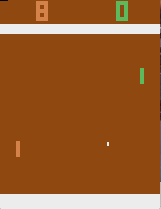
\includegraphics[scale=.9]{env.png}
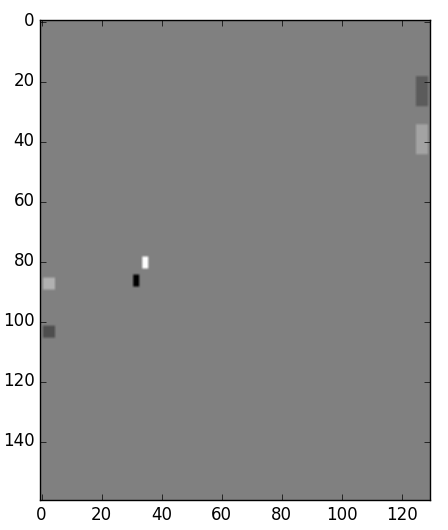
\includegraphics[scale=0.5]{df.png}
\end{figure}
\section{Implementation}
[4]
Line by line explanation of what the code does and looks like, how we realized Qlearning (decaying rate, epsilon, etc.)
\section{Results and Discussion}
\par
Final topology goes here
\par 
However, our algorithm is not performing as expected: the large majority of games played by our algorithm end in scoreless losses.  This could partially be due to a lack of exploration of the hyperparameter landscape because due to technical limitations, training time took too long to adequately evaluate the performance of a neural network with each possible configuration.  In addition, the technical limitations put a cap on how large of a network we could generate without running out of memory, and our topology reflects this upper limit.  It's possible that even though we have a large number of nodes, it's still insufficient to handle the massive amounts of input generated by the environment.
\par
However, our difficulties are also partially due to the realization of pong in OpenAI Gym's environment.  The environment has your AI faced against a premade AI that is quite good at returning shots.  One particular facet of the AI that has posed problems for learning is its service pattern, which alternates between one of two spots (one on top, one on bottom) depending on whether the player returned the serve or not.  Due to this pattern, we could see our algorithm learning to start by moving to either the very top and very bottom of the screen and then struggle to learn to move to the other side after several points of missing the ball, which was being served in the same spot on the other side of the screen.  We tried to alleviate this by suppressing the learning rate and implementing a decaying learning rate that would hopefully minimize the effect these service problems had on the weights it learned during earlier training sessions.  Ideally, if we had the ability to alter the environment provided to us by the OpenAI Gym we would have pitted our algorithm against a more fair opponent: itself.  At the very least, altering the service pattern so that it served in a random direction rather than in the same direction every time would have potentially allowed for our algorithm to learn more easily.
\par
The "Pong-v0" environment is not an impossible problem, and as a matter of fact, there exist several implementations that work well on the webpage of the problem[3], but the difference between these implementations and our own is that the neural networks they used were more sophisticated than what our computational resources could handle.  For example, one of the solutions uses a convolutional neural network[5], and while we attempted to train one of these networks, training time was incredibly slow (~1.5 minutes for 1 iterations, which translates to 2.5 hours for 100 iterations), and creating a network of any significant size resulted in running out of memory.  In summary, in order for success to be achieved on this project, either we needed to alter the problem (opposing player AI), or gain access to more computational resources, such as the supercomputer.
\section{Conclusion}

\section{References}
[1] https://gym.openai.com \newline
[2] https://gym.openai.com/envs/DoomBasic-v0 \newline
[3] https://gym.openai.com/envs/Pong-v0 \newline
[4] https://www.tensorflow.org \newline
[5] https://gym.openai.com/evaluations/eval\_Ce7x6ryRrCMB7JlpbQ \newline

\end{document}